
\section{Versailles}
Symbol velikosti krále a vlasti a vzor snad pro každého „zámeckého architekta“ Evropy – to jsou Versailles (obrázek ~\ref{ver1}). Když se Ludvík XIV. (1638–1715) rozhodl, že přestaví malý lovecký zámeček svého otce ve Versailles 20 kilometrů západně od Paříže na nádherný palác, bylo králi Slunce právě 23 let. Francouzští panovníci sídlili v Louvru od 13. století. Od roku 1661 se Versailles staly rezidencí a sídlem vlády a absolutním mocenským centrem Francie.\\\begin{figure}[h!]
\centering
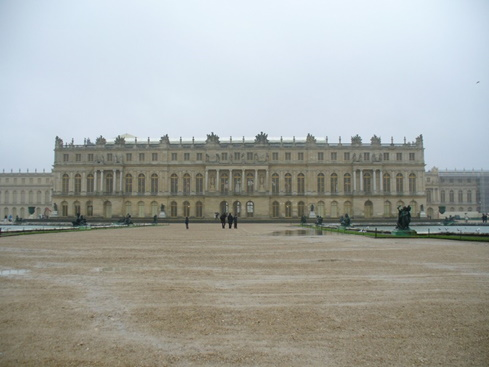
\includegraphics[scale=0.5]{images/obr10V.jpg}
\caption{Versailles}
\label{ver1}
\end{figure}\\Vše, co mohl francouzský národ nabídnout coby umělce a umělecké řemeslníky – celkem asi 30 000 lidí -, bylo posláno do Versailles, aby se podílelo na přestavbě feudálního zámku. Realizací celého díla pověřil král architekty La Vaua a Mansarta, interiérového architekta Le Bruna a zahradního architekta Le Notra. Trvalo celkem 50 let, než byl skvostný zámek dokončen tak, aby uspokojil ctižádostivost a vůli krále Slunce. Nejslavnějším a nejkrásnějším prostorem v zámeckém interiéru je Zrcadlový sál dokončený v roce 1684 a dlouhý 73 metrů. Z toho grandióuního místa dal Bismarck vyhlásit v roce 1871 Německé císařství. Uprostřed zámku je umístěna světoznámá přepychová ložnice krále. V ložnici královny, která už není tak velkolepá, přišlo na svět 19 princů a princezen.\\\\Za pozornost stojí i zahrady tohoto 680 metrů dlouhého zámku, které můžeme vidět na obrázku ~\ref{ver2}. Rozkládají se na více než 100 hektrech a musel splňovat právě tak vysoké reprezentační nároky jako sám zámek. Byly v nich vybudovány vyhlídky, široké aleje zdobené sochami a umělé kanály – „malé Benátky“. Během velkolepých barokních dvorských slavností se v parku konala operní představení. Zahradní zámek Grand Triaton, který v roce 1687 postavil Mansart, věnoval Ludvík XVI. Své manželce Marii Antoinettě. Malý zámeček Petit Trianon vznikl v roce 1762. marie Antoinetta si dala postavit i Le Hameau, vzorovou vesnici s lékárnou a mlýnem, kde se královna snažila napodobovat selský život. Za krále–občana Ludvíka Filipa v roce 1837 bylo ve Versailles zřízeno muzeum.\\\\K volné prohlídce jsou určeny Velké komnaty, Zrcadlová galerie, Galerie bitev a části obrazové galerie. Další prostory jsou přístupné jen s průvodcem.\cite{rodreguaze}

\begin{figure}[h!]
\centering
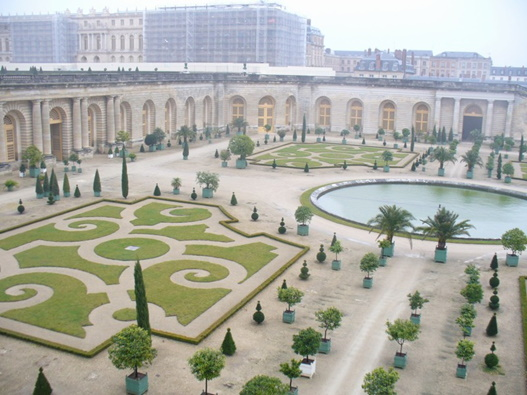
\includegraphics[scale=0.5]{images/obr11V.jpg}
\caption{Versailleský park}
\label{ver2}

\end{figure}
